\chapter{Conclusions and future work}
\label{ch:conclusion}

Lorem ipsum dolor sit amet, consectetur adipiscing elit. Duis tincidunt eros ut dictum tempor. Proin rhoncus elementum mauris, ac bibendum quam. Sed eget nisi non arcu malesuada pulvinar a at ipsum. Curabitur ante quam, aliquet id purus ac, interdum semper odio. Suspendisse potenti. Aliquam rhoncus massa consectetur faucibus condimentum. Sed euismod tellus eu mattis elementum. In nec laoreet ligula. Donec vel blandit ante. Mauris non ligula non justo venenatis rhoncus. In quis auctor ipsum, in mattis lacus. In vitae lectus sodales arcu iaculis bibendum. Fusce ornare at ex vitae ultricies.

\section{Future Work}
Lorem ipsum dolor sit amet, consectetur adipiscing elit. Duis tincidunt eros ut dictum tempor. Proin rhoncus elementum mauris, ac bibendum quam. Sed eget nisi non arcu malesuada pulvinar a at ipsum. Curabitur ante quam, aliquet id purus ac, interdum semper odio. Suspendisse potenti. Aliquam rhoncus massa consectetur faucibus condimentum. Sed euismod tellus eu mattis elementum. In nec laoreet ligula. Donec vel blandit ante. Mauris non ligula non justo venenatis rhoncus. In quis auctor ipsum, in mattis lacus. In vitae lectus sodales arcu iaculis bibendum. Fusce ornare at ex vitae ultricies.

\subsection{Computing multiple rectification functions}

Lorem ipsum dolor sit amet, consectetur adipiscing elit. Duis tincidunt eros ut dictum tempor. Proin rhoncus elementum mauris, ac bibendum quam. Sed eget nisi non arcu malesuada pulvinar a at ipsum. Curabitur ante quam, aliquet id purus ac, interdum semper odio. Suspendisse potenti. Aliquam rhoncus massa consectetur faucibus condimentum. Sed euismod tellus eu mattis elementum. In nec laoreet ligula. Donec vel blandit ante. Mauris non ligula non justo venenatis rhoncus. In quis auctor ipsum, in mattis lacus. In vitae lectus sodales arcu iaculis bibendum. Fusce ornare at ex vitae ultricies. Fig. \ref{fig:2bit_redbI}. 

\begin{figure}[htp]
    \centering
    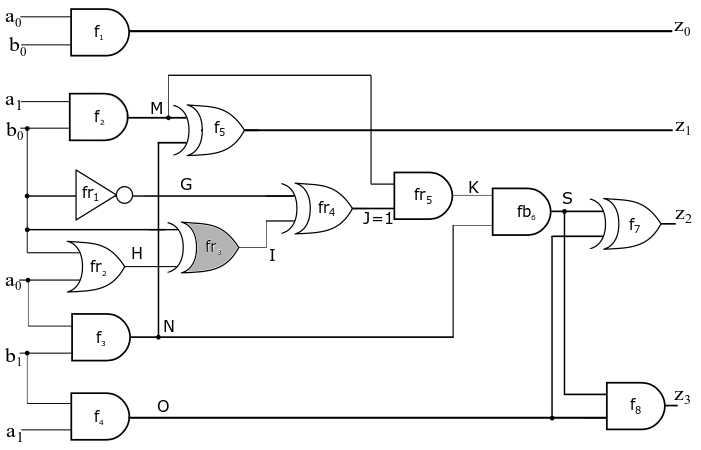
\includegraphics[scale = 0.5]{int2_red_bI.png}
    \caption{2-bit integer multiplier with redundancy. Bug at $I$.}
    \label{fig:2bit_redbI}
\end{figure}

The procedure to compute a rectification polynomial is applied and the polynomial $I = b_0$ is computed.

\subsection{Dependency constrained rectification function}

Lorem ipsum dolor sit amet, consectetur adipiscing elit. Duis tincidunt eros ut dictum tempor. Proin rhoncus elementum mauris, ac bibendum quam. Sed eget nisi non arcu malesuada pulvinar a at ipsum. Curabitur ante quam, aliquet id purus ac, interdum semper odio. Suspendisse potenti. Aliquam rhoncus massa consectetur faucibus condimentum. Sed euismod tellus eu mattis elementum. In nec laoreet ligula. Donec vel blandit ante. Mauris non ligula non justo venenatis rhoncus. In quis auctor ipsum, in mattis lacus. In vitae lectus sodales arcu iaculis bibendum. Fusce ornare at ex vitae ultricies.

\subsection{Impact of term orders on efficiency}

Lorem we discuss the limitation of \Grobner Basis reduction with Reverse Topological Term Order (RTTO) imposed on the variables. We witness the problem of variable explosion. Consider the example below, where \Grobner Basis reduction is performed with a forward topology based term order. 

\begin{Example}
Lorem ipsum dolor sit amet, consectetur adipiscing elit. Duis tincidunt eros ut dictum tempor. Proin rhoncus elementum mauris, ac bibendum quam. Sed eget nisi non arcu malesuada pulvinar a at ipsum. Curabitur ante quam, aliquet id purus ac, interdum semper odio. Suspendisse potenti. Aliquam rhoncus massa consectetur faucibus condimentum. Sed euismod tellus eu mattis elementum. In nec laoreet ligula. Donec vel blandit ante. Mauris non ligula non justo venenatis rhoncus. In quis auctor ipsum, in mattis lacus. In vitae lectus sodales arcu iaculis bibendum. Fusce ornare at ex vitae ultricies.
\end{Example}

\subsection{Multi-fix rectification}

Not all the bugs that may be present in a circuit can be rectified at a single location. Some bugs can be rectified only by the implementation of multiple functions at multiple nets in the circuit. 

